\documentclass{article} 
\usepackage[polish]{babel}
\usepackage[utf8]{inputenc}	
\usepackage{polski}	
\usepackage[T1]{fontenc}
\frenchspacing	
\usepackage{indentfirst}
\usepackage{fancybox} 
\usepackage{geometry}
\geometry{
	total={170mm,250mm},
	left=20mm,
	top=20mm,
}
\usepackage{multirow}
\usepackage{graphicx}
\usepackage{array}
\usepackage{makecell}
\usepackage{listings}
\lstdefinestyle{gitstyle}{
	basicstyle=\ttfamily\small,
	keywordstyle=\color{blue},
	commentstyle=\color{Gray},
	backgroundcolor=\color{Gray},
	frame=single,
	rulecolor=\color{black},
	breaklines=true,
	showstringspaces=false,
	tabsize=2,
	numbers=left,
	numberstyle=\tiny\color{Gray},
	xleftmargin=2em,
	framexleftmargin=1.5em
}
\lstset{style=gitstyle}
\usepackage{color, colortbl}
\definecolor{Gray}{gray}{0.9}
\usepackage{lipsum}
\usepackage[compact]{titlesec}
\titleformat{\subsection}[runin]
{\normalfont\large\bfseries}{\thesubsection}{1em}{}[{\\[0,5em]}]
\titlespacing*{\subsection}{1cm}{1em}{0em}
\newcommand{\forceindent}{\leavevmode{\parindent=1cm\indent}} %



\def\AuthorFirstName{JAROSŁAW}
\def\AuthorLastName{Pytlik}
\def\Title{Zaliczenie}
\def\DateOfExecution{2026-06-14}
\def\DateOfDeliver{2026-06-14}
%
%
\begin{document}	
	\noindent
	\def\arraystretch{1.5} \small
	\begin{table}
		\resizebox{\textwidth}{!}{\begin{tabular}{|p{2.6cm}|p{4cm}|p{3cm}|p{3cm}|l|}
		\hline 
		\multirow{4}{2.6cm}{\centering
\includegraphics[width=1.40cm]{image/ModLogoPO}\\[0.05cm]
\includegraphics[width=1.40cm]{image/ModLogoWE}} & PRZEDMIOT: & \multicolumn{3}{l|}{ \makecell[l]{\noalign{\vskip3pt}PRZEDMIOT WYBIERALNY XIV:\\ NARZ\k{E}DZIA INFORMATYCZNE W PRAKTYCE \\IN\.{Z}YNIERSKIEJ}}\tabularnewline
		\cline{2-5} \cline{3-5} \cline{4-5} \cline{5-5} 
		& KIERUNEK STUDIÓW: & INFORMATYKA & ROK STUDIÓW: & IV\tabularnewline
		\cline{2-5} \cline{3-5} \cline{4-5} \cline{5-5} 
		& ROK AKADEMISKI: & 2025/2026 & SEMESTR: & 8\tabularnewline
		\cline{2-5} \cline{3-5} \cline{4-5} \cline{5-5} 
		& TEMAT: & \multicolumn{3}{l|}{\makecell[l]{\noalign{\vskip3pt} \Title }}\tabularnewline
		\hline 
		IMI\k{E}: & \textbf{\AuthorFirstName} & \multicolumn{2}{l|}{DATA WYKONANIA \'{C}WICZENIA: }  & \DateOfExecution \tabularnewline
		\hline 
		NAZWISKO: & \textbf{\AuthorLastName} & \multicolumn{2}{l|}{DATA ODDANIA SPRAWOZDANIA:} & \DateOfDeliver \tabularnewline
		\hline 
		OCENA: & DATA: & \multicolumn{3}{l|}{UWAGI}\tabularnewline
		\hline \rowcolor{Gray}
		{\makecell[l]{ \\ \\ \\ \\}}&  & \multicolumn{3}{l|}{}\tabularnewline
		\hline 
		\end{tabular}}
	\end{table}
% POCZĄTEK SPRAWOZDANIA
	
	\section{Zadanie 1}
	\begin{figure}[h]
		\centering
		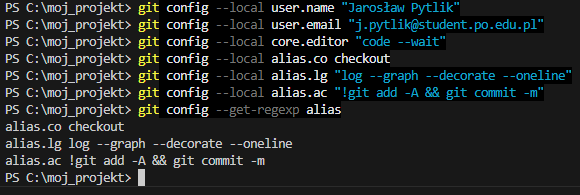
\includegraphics[width=0.8\textwidth]{image/1.png}
	\end{figure}
    \newpage
    \section{Zadanie 2}
	\begin{figure}[h]
		\centering
		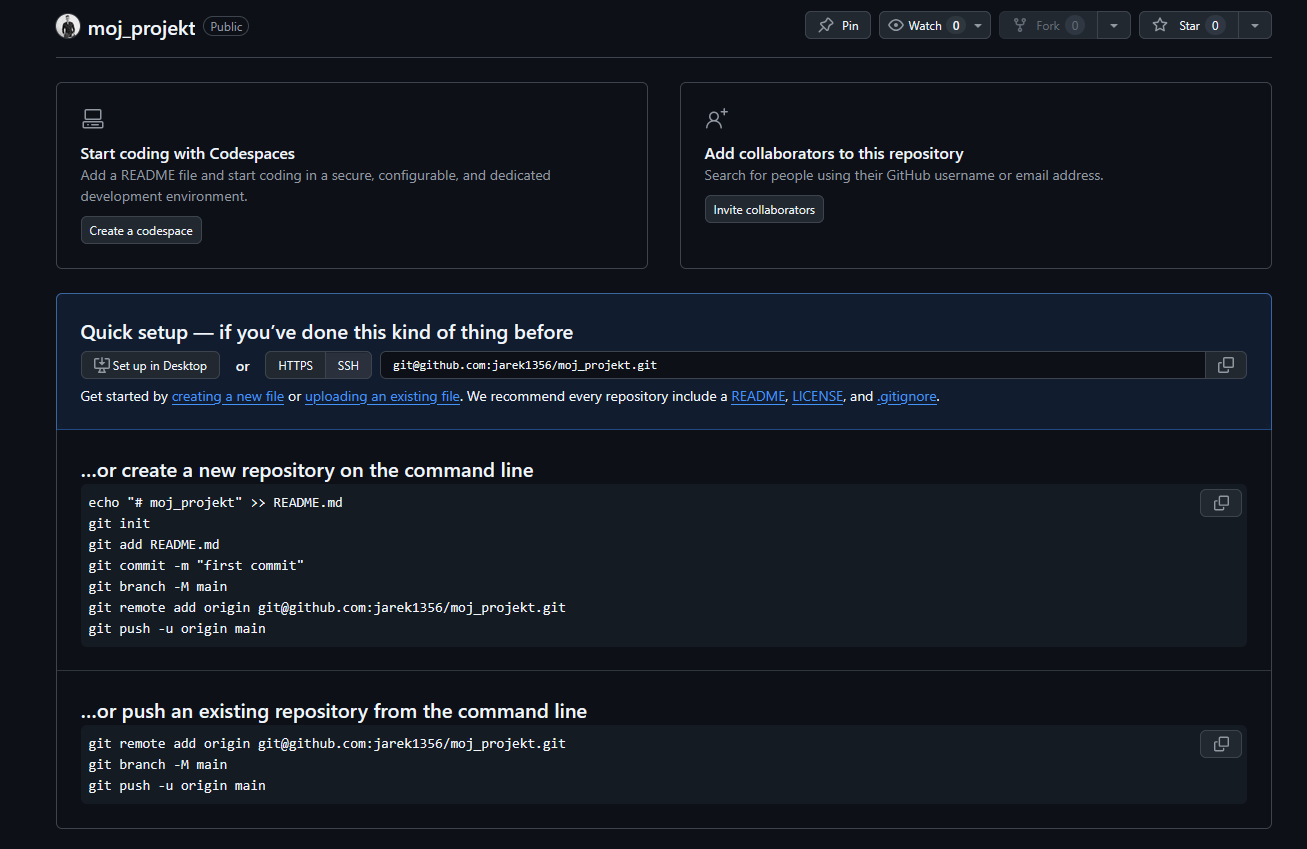
\includegraphics[width=0.8\textwidth]{image/2.png}
	\end{figure}
    \section{Zadanie 3}
	\begin{lstlisting}
PS C:\moj_projekt> git branch -M main
PS C:\moj_projekt> git remote add origin git@github.com:jarek1356/moj_projekt.git
PS C:\moj_projekt> git fetch origin
PS C:\moj_projekt> git log --oneline --graph --decorate --all
* afa4b01 (HEAD -> main) Pierwszy commit
PS C:\moj_projekt> git push -u origin main
PS C:\moj_projekt> git add .
PS C:\moj_projekt> git commit -m "ADD LINK GITHUB IN README.MD" 
PS C:\moj_projekt> git push -u origin main   
	\end{lstlisting}

    \section{Zadanie 3}
    	\begin{lstlisting}
PS C:\moj_projekt> git status
On branch main
Your branch is up to date with 'origin/main'.

Untracked files:
  (use "git add <file>..." to include in what will be committed)
        .gitignore

nothing added to commit but untracked files present (use "git add" to track)
	\end{lstlisting}
		

	
	
\end{document}	
